\section{Introduction}

% Start with a little story
\begin{center}
  \fbox{
    \parbox{0.85\linewidth}{
    \noindent
    \emph{``What did you see in this image?''\\
      ``Panda, Tiger, Elephant, Lions.''\\
      ``Have you seen the Gorilla?''\\
      ``Oh! I even didn't notice there is a Gorilla !''}
    }
  }
\end{center}

\setlength{\tabcolsep}{2pt}
\begin{figure}[htb]
\begin{center}
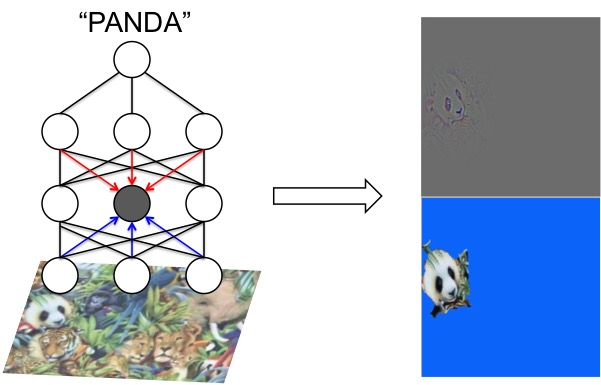
\includegraphics[width=0.95\columnwidth]{figs/splash0/splash}
% \vspace{-10pt}
\caption{We propose a novel Feedback Convolutional Net model for captuing visual attention by infering the status of hidden neuron activations. The feedback net is designed to utilize both bottom-up image features and top-down semantic labels to infer the hidden neuron activations. The salient area captured by feedback often matches the correponding "target" object, even in the images with cluttered background and multiple objects.}
\label{fig:splash0}
\vspace{-10pt}
\end{center}
\end{figure}

Visual attention typically is dominated by \emph{``goals''} from our mind easily in a top-down manner, especially in the case of object detection. Cognitive science explains this in the ``Biased Competition Theory''~\cite{beck2009top,desimone1998visual,desimone1995neural}, that human visual cortex is enhanced by top-down stimuli and non-relevant neurons will be suppressed in feedback loops when searching objects. By ``looking and thinking twice'', both human recognition and detection performances increase significantly especially in images with cluttered background~\cite{Cichy2014Resolving}. This leads to the selectivity in neuron activations~\cite{Kruger2013Deep}, which reduces the chance of recognition being interfered with either noises or distractive patterns.

Inspired by the above evidences, we present a novel \emph{Feedback Convolutional Neural Network} architecture in this paper. It achieves this selectivity by jointly reasoning the outputs of class nodes and the activations of hidden layer neurons during the feedback loop. As shown in Figure~\ref{fig:splash0}, during the feedforward stage, the proposed networks perform inference from image features in a bottom-up manner as traditional Convolutional Networks; while in feedback loops, it sets up high-level semantic labels (\emph{e.g.}, outputs of class nodes) as the ``goal'' in visual search to infer the activation status of hidden layer neurons. The networks are powerful enough to apply for class model visualization~\cite{simonyan2013deep, zeiler2014visualizing} and object localization even in cluttered scenes with multiple objects.

\setlength{\tabcolsep}{0.5pt}
\begin{figure*}[htb]
\begin{center}
\begin{tabular}{ccccccc}
%\rotatebox{90}{\hspace{5mm}Sequential} &
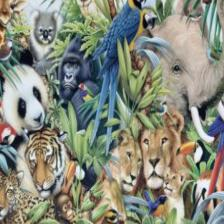
\includegraphics[width=0.14\linewidth]{figs/splash/original} &
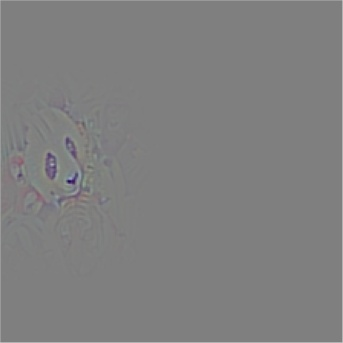
\includegraphics[width=0.14\linewidth]{figs/splash/panda} &
\includegraphics[width=0.14\linewidth]{figs/splash/tiger} &
\includegraphics[width=0.14\linewidth]{figs/splash/gorilla} &
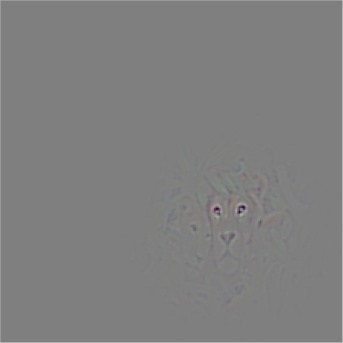
\includegraphics[width=0.14\linewidth]{figs/splash/lion} &
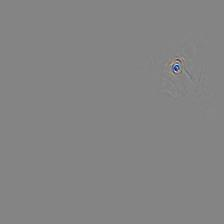
\includegraphics[width=0.14\linewidth]{figs/splash/elephant} &
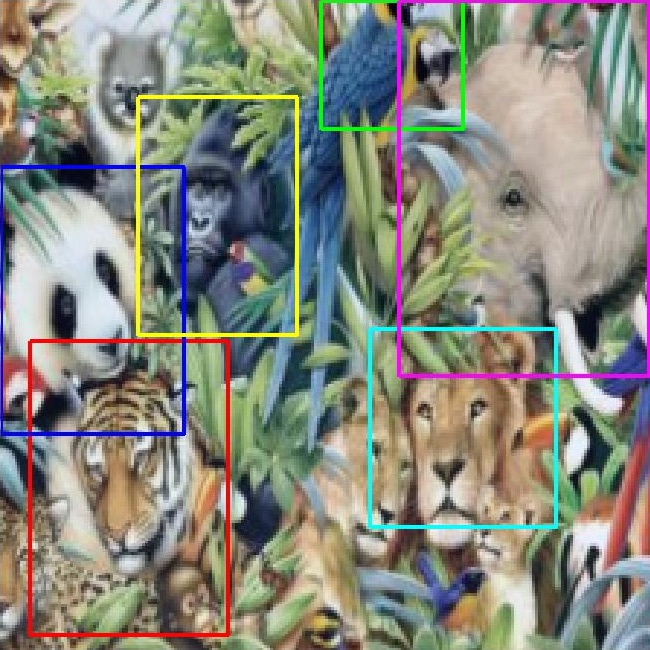
\includegraphics[width=0.14\linewidth]{figs/splash/localization}\\
{\small (a) Input Image} &
{\small (b) Panda} &
{\small (c) Tiger} &
{\small (d) Gorilla} &
{\small (e) Lion} &
{\small (f) Elephant} &
{\small (g) Localization}
\end{tabular}
% \vspace{-10pt}
\caption{We illustrate the localization power of the feedback net on a multi-object image with cluttered background. (a) shows the original input image which both VggNet and GoogleNet recongize as "comic book". (b) - (f) illustrate our feedback modelon understanding the image given different class labels as a prior. We visualize the gradient of each class node with respect to image after the feedback net finish its inference. (g) shows the final localizations for different objects based on the gradients. Better viewed in color.}
\label{fig:splah}
% \vspace{-30pt}
\end{center}
\end{figure*}

\subsection{Optimization in a Feedback Loop}
% Explain from the machine learning perspective
From a machine learning perspective, the proposed feedback networks \emph{add extra flexibility to Convolutional Networks, to help in capturing visual attention and improving feature detection}. Convolutional Neural Networks~\cite{lecun1998gradient, Krizhevsky2012ImageNet, Simonyan2014Very} have achieved great success in both machine learning and computer vision recent years. Benefit from large scale of training data, (\emph{e.g.,} ImageNet~\cite{deng2009imagenet}), CNNs are capable of learning filters and image compositions at the same time. Various approaches have been adopted to further increase ability of CNN, by either adding regularization in training~\cite{he2015delving,ioffe2015batch}, or going deeper~\cite{Simonyan2014Very, Szegedy2014Going}. Inspired by the Deformable Part-Based Models (DPM)~\cite{Felzenszwalb2010Object} that model middle level part locations as latent variables and search for them during object detection, we utilize a simple yet efficient method to optimize image compositions and assign neuron activations given ``goals'' in visual searching. The algorithm maximizes the posterior response of network given target high-level semantic concepts, in a top-down manner. Compared with traditional bottom-up strategies~\cite{he2015delving, ioffe2015batch} which aim to regularize the network training, the proposed feedback framework adds flexibilities to the model inference from high-level concepts down to receptive fields.

As the example shown in Figure~\ref{fig:splash0}, given a high-level semantic stimulus ``PANDA'', only the neurons in hidden layers related with the concept ``PANDA'' will be activated by iterative optimization in a feedback loop. As a result, only salient regions related with the concept ``PANDA'' are captured in visualizations. Figure~\ref{fig:splah} also shows the visualizations of saliencies given different semantic concepts for the same input image. As suggested by those results, the feedback networks achieve certain level of selectivity and provide non-relevant suppression during the top-down inference, allowing the model to focus on the most importatn image regions that improve the class confidence. 

%Comparisons between our method against two other visualization algorithms, Oxford~\cite{simonyan2013deep} and Deconvolution~\cite{zeiler2014visualizing}, are shown in Figure~\ref{fig:examples} in Section~\ref{sec:experiment}. Compared with state-of-the-arts, our feedback framework is capable to allow the model focusing on the most important image areas that improve the class confidence.

\subsubsection*{Weakly Supervised Object Localization}
% Unify the network: recognition and detection in a single network.
% Simultaneously answer the question of "what" and "where"
Given the gradient visualizations shown in Figure~\ref{fig:splah}, we further develop a weakly supervised object localization algorithm. Instead of using large amount of supervision (\emph{e.g.}, bounding box positions) in traditional methods such as R-CNN~\cite{girshick2014rich} or using regression model~\cite{erhan2014scalable, Simonyan2014Very}, we don't require any localization information in the training stage. In this case, we utilize \emph{a unified network performing both recognition and localization tasks}, to answer questions of ``what'' and ``where'' simultaneously, which are the two most important tasks in computer vision. Experimental results show that our weakly supervised algorithm using feedback network could achieve similar performance on ImageNet object localization task as GoogLeNet~\cite{Szegedy2014Going} and VGG~\cite{Simonyan2014Very}.

The remainder of this paper is organized as follows: Section~\ref{sec:related_work} introduces the related work, while we formulate our algorithm in Section~\ref{sec:model}. Experiments of visualization and object localization are demonstrated in Section~\ref{sec:experiment}. We conclude this work and future directions in Section~\ref{sec:conclusion}

% Implementation - caffe~\cite{jia2014caffe}



\begin{comment}

We present a novel feedback neural networks for joint reasoning the class node and hidden layer information. The network is powerful to be applied on model class visualization and object localization even in cluttered scenes with multi objects. The framework is novel and

\textbf{Deep Learning and Deep Convolutional Neural Networks, Feedforward Strcture}
Deep Convolutional networks (ConvNets) have recently enjoyed a great success in large-scale im- age and video recognition (Krizhevsky et al., 2012; Zeiler Fergus, 2013; Sermanet et al., 2014; Simonyan Zisserman, 2014) which has become possible due to the large public image reposito- ries, such as ImageNet (Deng et al., 2009), and high-performance computing systems, such as GPUs or large-scale distributed clusters (Dean et al., 2012). In particular, an important role in the advance of deep visual recognition architectures has been played by the ImageNet Large-Scale Visual Recog- nition Challenge (ILSVRC) (Russakovsky et al., 2014), which has served as a testbed for a few generations of large-scale image classification systems, from high-dimensional shallow feature en- codings (Perronnin et al., 2010) (the winner of ILSVRC-2011) to deep ConvNets (Krizhevsky et al., 2012) (the winner of ILSVRC-2012).

\textbf{Psychological feedback, inference top-down and bottom-up}
While we have outlined in this paper a hierarchical feedfor- ward view on visual processing, it is important to remember that within the visual cortex there are generally more feedback connections than forward connections. Also lateral connec- tions play an important role. This hints at the importance of processes like attention, expectation, top-down reasoning, imagination, and filling in. Many computer vision systems try to work in a purely feed-forward fashion. However, vision is inherently ambiguous and benefits from any prior knowledge available. This may even imply that the knowledge of how the tower of Pisa looks influences the perception of an edge on the level of V1. It also means that a system should be able to produce several hypotheses that are concurrently considered and possibly not resolved [102].

\textbf{This paper Main Contribution}
In this paper, we address the visualisation of deep image classification ConvNets, trained on the large-scale ImageNet challenge dataset [2]. To this end, we make the following three contributions. First, we demonstrate that understandable visualisations of ConvNet classification models can be ob- tained using the numerical optimisation of the input image [5] (Sect. 2). Note, in our case, unlike [5], the net is trained in a supervised manner, so we know which neuron in the final fully-connected clas- sification layer should be maximised to visualise the class of interest (in the unsupervised case, [9] had to use a separate annotated image set to find out the neuron responsible for a particular class). To the best of our knowledge, we are the first to apply the method of [5] to the visualisation of ImageNet classification ConvNets [8]. Second, we propose a method for computing the spatial support of a given class in a given image (image-specific class saliency map) using a single back-propagation pass through a classification ConvNet (Sect. 3). As discussed in Sect. 3.2, such saliency maps can be used for weakly supervised object localisation. Finally, we show in Sect. 4 that the gradient-based visualisation methods generalise the deconvolutional network reconstruction procedure [13].

\textbf{Yurgen's feedback neural networks, Attention neural networks, Deep Boltzman Machines}

\textbf{DPM  Top-down, weakly supervised object detection, localization and parsing}
We describe an object detection system that represents highly variable objects using mixtures of multiscale de- formable part models. These models are trained using a discriminative procedure that only requires bounding boxes for the objects in a set of images. The resulting system is both efficient and accurate, achieving state-of- the-art results on the PASCAL VOC benchmarks [11]– [13] and the INRIA Person dataset [10].
Our approach builds on the pictorial structures frame- work [15], [20]. Pictorial structures represent objects by a collection of parts arranged in a deformable configu- ration. Each part captures local appearance properties of an object while the deformable configuration is charac- terized by spring-like connections between certain pairs of parts.
Detections obtained with a single component person model. The model is defined by a coarse root filter (a), several higher resolution part filters (b) and a spatial model for the location of each part relative to the root (c). The filters specify weights for histogram of oriented gradients features. Their visualization show the positive weights at different orientations. The visualization of the spatial models reflects the “cost” of placing the center of a part at different locations relative to the root.

\textbf{Comparing against Oxford and Deconv}

\textbf{ConvNet Implementation Details}
ConvNet implementation details. Our visualisation experiments were carried out using a single deep ConvNet, trained on the ILSVRC-2013 dataset [2], which includes 1.2M training images, labelled into 1000 classes. Our ConvNet is similar to that of [8] and is implemented using their cuda-convnet toolbox1, although our net is less wide, and we used additional image jittering, based on zeroing-out random parts of an image. Our weight layer configuration is: conv64-conv256- conv256-conv256-conv256-full4096-full4096-full1000, where convN denotes a convolutional layer with N filters, fullM – a fully-connected layer with M outputs. On ILSVRC-2013 validation set, the network achieves the top-1/top-5 classification error of 39.7%/17.7%, which is slightly better than 40.7%/18.2%, reported in [8] for a single ConvNet.

\end{comment}

%\setlength{\tabcolsep}{2pt}
%\begin{figure*}
%\begin{center}
%\begin{tabular}{ccccccccc}
%\rotatebox{90}{\hspace{5mm}Oxford} &
%\includegraphics[width=0.11\linewidth]{figs/visual_compare/gradient/oxford/panda} &
%\includegraphics[width=0.11\linewidth]{figs/visual_compare/saliency/oxford/panda} &
%\includegraphics[width=0.11\linewidth]{figs/visual_compare/gradient/oxford/tiger} &
%\includegraphics[width=0.11\linewidth]{figs/visual_compare/saliency/oxford/tiger} &
%\includegraphics[width=0.11\linewidth]{figs/visual_compare/gradient/oxford/gorilla} &
%\includegraphics[width=0.11\linewidth]{figs/visual_compare/saliency/oxford/gorilla} &
%\includegraphics[width=0.11\linewidth]{figs/visual_compare/gradient/oxford/lion} &
%\includegraphics[width=0.11\linewidth]{figs/visual_compare/saliency/oxford/lion} \\
%\rotatebox{90}{\hspace{5mm}Deconv} &
%\includegraphics[width=0.11\linewidth]{figs/visual_compare/gradient/deconv/panda} &
%\includegraphics[width=0.11\linewidth]{figs/visual_compare/saliency/deconv/panda} &
%\includegraphics[width=0.11\linewidth]{figs/visual_compare/gradient/deconv/tiger} &
%\includegraphics[width=0.11\linewidth]{figs/visual_compare/saliency/deconv/tiger} &
%\includegraphics[width=0.11\linewidth]{figs/visual_compare/gradient/deconv/gorilla} &
%\includegraphics[width=0.11\linewidth]{figs/visual_compare/saliency/deconv/gorilla} &
%\includegraphics[width=0.11\linewidth]{figs/visual_compare/gradient/deconv/lion} &
%\includegraphics[width=0.11\linewidth]{figs/visual_compare/saliency/deconv/lion} \\
%\rotatebox{90}{\hspace{5mm}Our} &
%\includegraphics[width=0.11\linewidth]{figs/visual_compare/gradient/feedback/panda} &
%\includegraphics[width=0.11\linewidth]{figs/visual_compare/saliency/feedback/panda} &
%\includegraphics[width=0.11\linewidth]{figs/visual_compare/gradient/feedback/tiger} &
%\includegraphics[width=0.11\linewidth]{figs/visual_compare/saliency/feedback/tiger} &
%\includegraphics[width=0.11\linewidth]{figs/visual_compare/gradient/feedback/gorilla} &
%\includegraphics[width=0.11\linewidth]{figs/visual_compare/saliency/feedback/gorilla} &
%\includegraphics[width=0.11\linewidth]{figs/visual_compare/gradient/feedback/lion} &
%\includegraphics[width=0.11\linewidth]{figs/visual_compare/saliency/feedback/lion} \\
%&
%\multicolumn{2}{c}{{\small (a) Panda}} &
%\multicolumn{2}{c}{{\small (b) Tiger}} &
%\multicolumn{2}{c}{{\small (c) Gorilla}} &
%\multicolumn{2}{c}{{\small (d) Lion}} \\
%\end{tabular}
%% \vspace{-10pt}
%\caption{We demonstrate the effectiveness of our method by comparing the class model visualization results against Oxford~\cite{simonyan2013deep} and Deconv~\cite{zeiler2014visualizing}. The input image is the same as Figure 1 (a). We show both the visualization results as well as the saliency map. While both Oxford and Deconv have the same input: the image and an object class label (i.e. tiger, panda, etc.), the gradients computed are often salient on one particular object (i.e. elephant). Our feedback framework allows for the model to focus on the most important image area that improves the class confidence.}
%\label{fig:visual_compare}
%% \vspace{-30pt}
%\end{center}
%\end{figure*}
